\subsection{Safety Surveillance Specification}
 In this example, we demonstrate the behaviour of the agent under a safety surveillance specification. We do so in the urban environment illustrated in Figure~\ref{fig:UE4city}. 
 
\begin{figure}
\centering
\subfloat[Top-down view of environment from Figure \ref{fig:UE4city}. The red square corresponds to the area in which the simulation takes place. \label{fig:topdownviewAirsim}]{
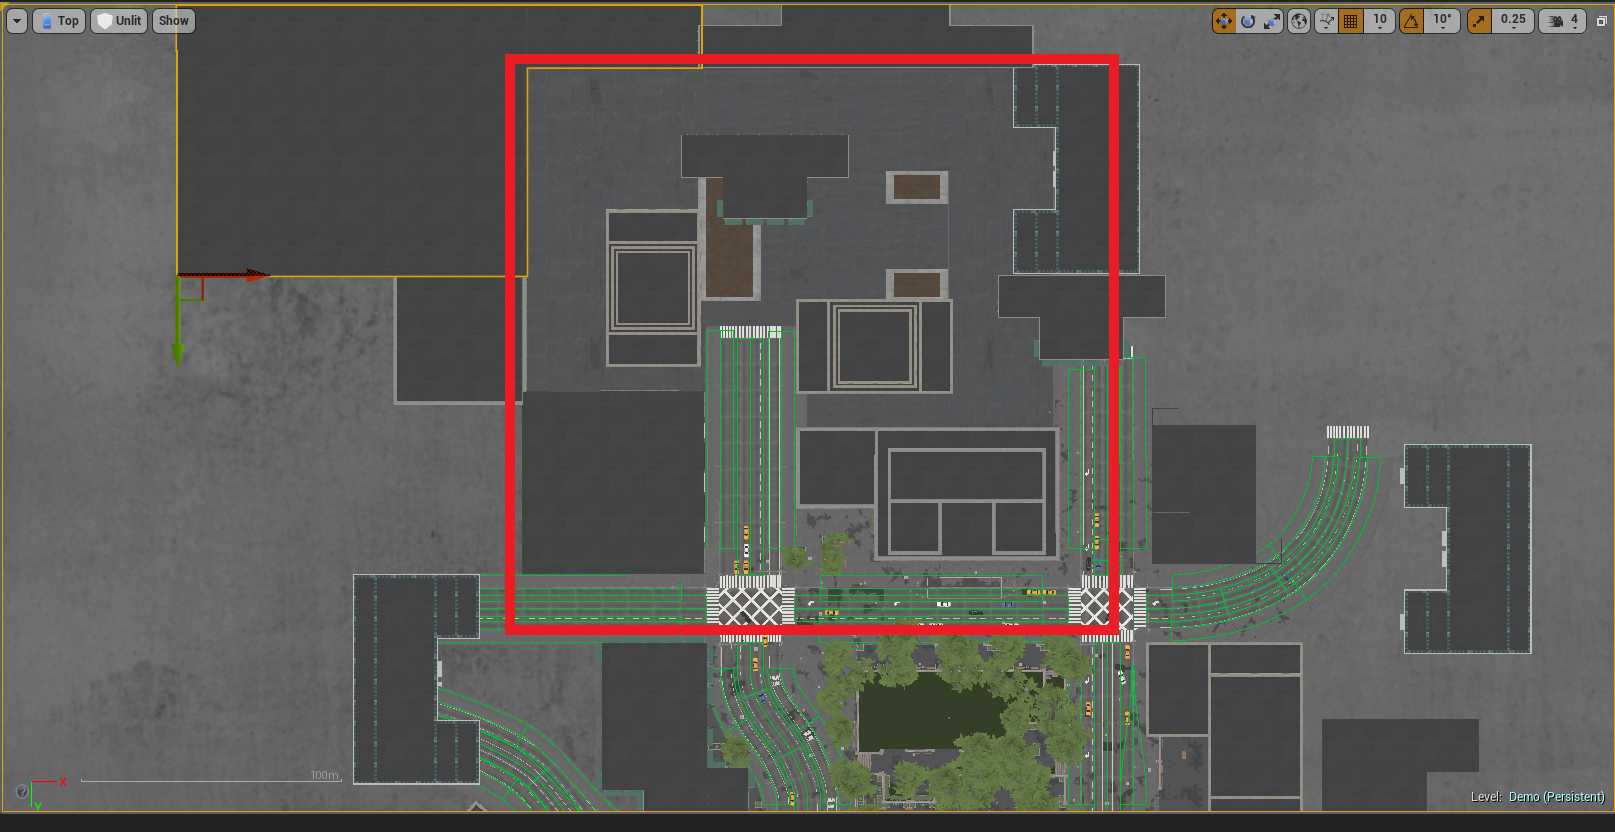
\includegraphics[width = 0.95\linewidth]{Surveillance/figs/downtown_map.png}}

\subfloat[The environment in \ref{fig:UE4city} is discretized into a 24x37 grid. Black cells are states that cannot be sensed from the current location of the agent. The agent is shown in blue, the evading target in orange. \label{fig:Airsim_grid}]{
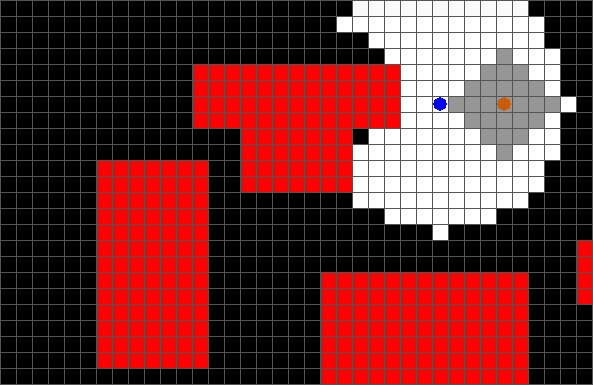
\includegraphics[width = 0.9\linewidth]{Surveillance/figs/Airsim_gridAirsim_Example.png}
}

\caption{The urban environment in Figure \ref{fig:GazArena} is discretized in \ref{fig:Airsim_grid} for synthesis. Note that due to the sensor uncertainty, the agent does not know the exact location of the target even when it is in range of its sensors.}
\label{fig:Airsim_casestudy}
\end{figure}
Figure~\ref{fig:Airsim_casestudy} depicts the top-down view environment created in \emph{Unreal Engine 4} and discretized for synthesis. The uncertainty in the sensing capaiblities of the agent is shown in Figure~\ref{fig:Airsim_grid} where grey cells correspond to the agent's current belief of the target's location stemming from the sensor and target state estimation uncertainty. The agent is 3 times faster than the target (it can move 3 cells for every 1 cell the target moves). 

In this setting, we require the satisfaction of the safety surveillance objective $\square p_{25}$ (the belief size should never exceed 25). In this case, we only need an abstraction with a trivial abstraction partition, consisting of the whole set of locations, as the agent has a strategy to closely follow and maintain view of the target. This is, in fact, necessary, as
any belief state will already be violating the safety requirement due to the estimation uncertainty. We are able to synthesize a strategy in 112 seconds. 
 
We present a video from the first-person view of the surveilling drone at \url{https://www.youtube.com/watch?v=HLsZ5ZnQgAg}. We note that the agent follows the target closely and never allows the target to leave its line of sight. In general, open urban environments the one considered here require stricter surveillance specifications as it is much harder to `find' a target once it has been lost. This will be in contrast with the more enclosed locations which we consider in the next case study.




\subsection{Liveness Surveillance Specification and Task Requirement} 
In this experiment, we demonstrate the behaviour an automatically synthesized strategy for the surveillance agent under a liveness surveillance specification and a task requirement. We do so in the Gazebo environment shown in Figure~\ref{fig:GazArena}. We compare this to a strategy for a safety surveillance specification with no additional task requirement, synthesized for the same environment. 



\begin{figure}
\subfloat[Lidar generated map of the gazebo environment in Figure~\ref{fig:GazArena}. \label{fig:Q_building_2}]{
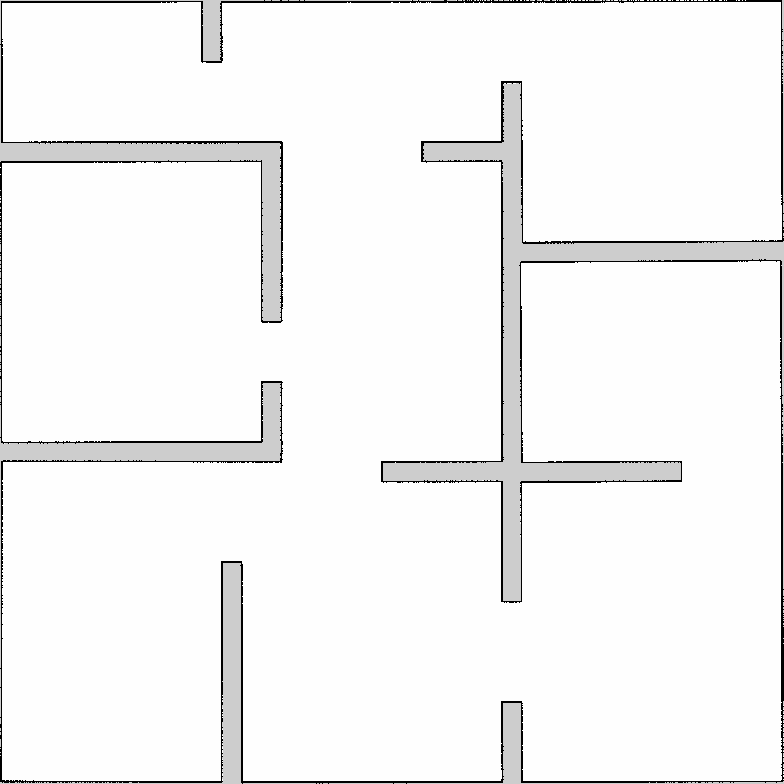
\includegraphics[width=0.45\linewidth]{Surveillance/figs/Q_building_2.png}
}
\hspace{0.5cm}
\subfloat[Discretization of the map \newline in Figure~\ref{fig:Q_building_2} used for synthesis \label{fig:gazebogrid}]{
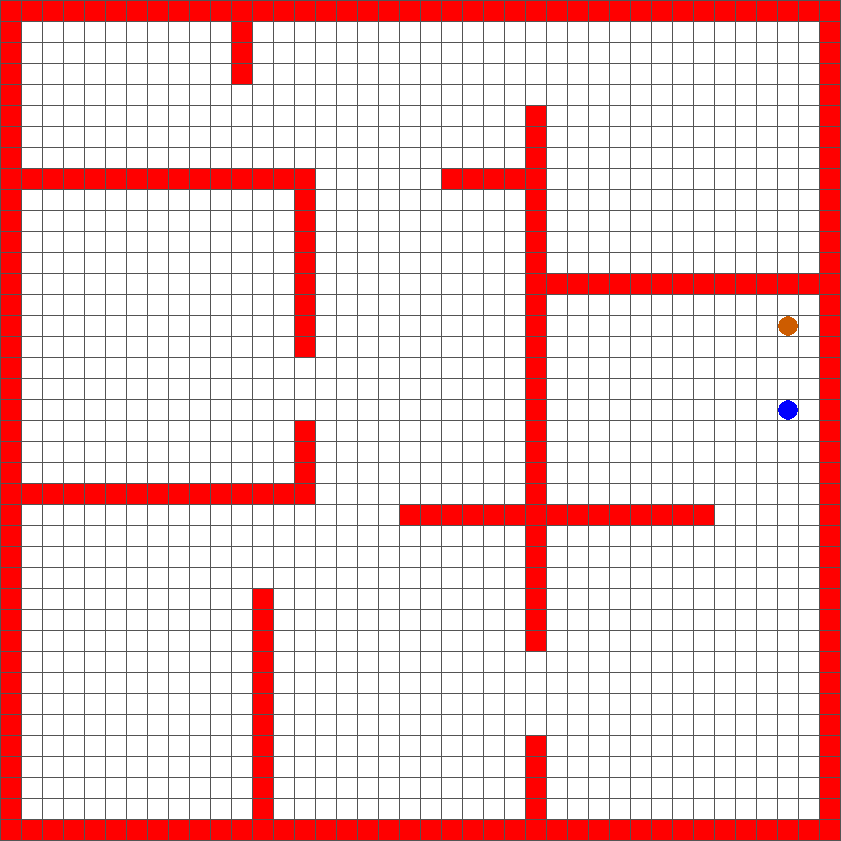
\includegraphics[width=0.45\linewidth]{Surveillance/figs/ROS_grid.png}\hspace{.5cm}
}

\caption{The Gazebo environment in Figure \ref{fig:GazArena} is first mapped using a LIDAR equipped agent to produce the map in~\ref{fig:Q_building_2} and then discretized to produce the gridworld in~\ref{fig:gazebogrid}.}
\label{fig:casestudiesros}

\end{figure}


The Iris quadcoptor shown in Figure~\ref{fig:sandiauav} is the agent being controlled by the synthesized surveillance strategy, and the Stanley Innovations Segway in Figure~\ref{fig:stanleyrobot} is the target. The target can either be controlled through a Python API or joystick such as an XBOX 360 controller. The quadcoptor uses a minimum snap trajectory package to plan its path, and a standard PX4 flight stack for the lower level flight control \cite{px4}. As in the previous section, we assume that the quadcoptor can move 3 times faster than the segway.

\begin{figure}[h]
  \definecolor{bg}{HTML}{ddeedd}
\definecolor{comp}{HTML}{c2d4dd}
\definecolor{impl}{HTML}{b0aac0}
\definecolor{ligb}{HTML}{5E7FC6}
\definecolor{bodybl}{HTML}{85A1DC}
\definecolor{headbl}{HTML}{264C9C}
\definecolor{bgyel}{HTML}{FFDC6B}
\definecolor{bodyyel}{HTML}{FFE58F}
\definecolor{headyel}{HTML}{E9BB25}
\definecolor{gr1}{HTML}{00FF00}
\definecolor{or1}{HTML}{FFAA00}
\definecolor{ye1}{HTML}{FFFF00}

% Define block styles
\tikzstyle{decision} = [diamond, draw, fill=blue!20, 
text width=4.5em, text badly centered, node distance=3cm, inner sep=0pt]
\tikzstyle{block} = [rectangle, draw, fill=blue!20, 
text width=5em, text centered, rounded corners, minimum height=4em]
\tikzstyle{line} = [draw, -latex']
\tikzstyle{cloud} = [draw, ellipse,fill=red!20, node distance=3cm,
minimum height=2em]
\def\checkmark{\tikz\fill[scale=0.6](0,.35) -- (.25,0) -- (1,.7) -- (.25,.15) -- cycle;} 
%
\centering
\begin{tikzpicture}[every node/.style={draw, text centered, shape=rectangle, rounded corners, text width=3cm, minimum height=0.8cm, inner sep=5pt}]
%\tikzstyle{outer}= [draw, text centered, shape=rectangle, text width=2cm, minimum height=1cm]
%\tikzstyle{inner}=[draw, text centered, shape=rectangle, rounded corners, text width=3.8cm, minimum height=1.1cm, inner sep=5pt]
\tikzstyle{decision} = [diamond, draw, aspect=3 , inner sep=3pt]


\node[fill=gr1!20!white] (launch){Launch};
\node[below=0.5cm of launch,fill=gr1!20!white] (move) {Flight};
\node[fill=blue!10!white,decision,below=0.5cm of move] (range) {Within range?};
\node[below=0.5cm of range,fill=or1!20!white] (loiter) {Loiter};
\node[fill=blue!10!white,decision,below=0.5cm of loiter] (assign) {Assigned?};
\node[below=0.5cm of assign,fill=ye1!20!white] (approach) {Approach};
\node[right=0.5cm of approach,fill=red!20!white,text width=1.5cm,inner sep=1pt] (land) {Land};

\path [line,-latex',very thick] (launch.south) -- (move.north);
\path [line,-latex',very thick] (move.south) -- (range.north);
\path [line,-latex', very thick] (range.south) --node[draw=none,right=-1.2cm]{Yes} (loiter.north);
\path [line,-latex', very thick] (range.east) -- node[draw=none,above=1pt] {No} ++(1.0,0)   |- (move.east);
\path [line,-latex', very thick] (loiter.south) --node[draw=none,left=-1cm]{Request} (assign.north);
\path [line,-latex', very thick] (assign.south) --node[draw=none,right=-1.2cm]{Land} (approach.north);
\path [line,-latex', very thick] (assign.east)  -- node[draw=none,above=1pt] {No} ++(1.0,0) |- (loiter.east);
\path [line,-latex', very thick] (assign.west)  -- node[draw=none,below=1pt] {Pass-through} ++(-1.0,0) |- (move.west);
\path [line,-latex', very thick] (approach.east) -- (land.west);


\end{tikzpicture}
    \caption{Flow chart of general procedure to synthesize surveillance strategies in Gazebo worlds and simulate the resulting strategies.}
    \label{fig:Flowmap}
\end{figure}


The Gazebo world is created using the building editor feature. An occupancy map of the world is created using the ROS Gmapping package. The Segway is manually driven around during mapping to generate the LIDAR map shown in Figure~\ref{fig:Q_building_2}. This map is then discretized to the map shown in Figure \ref{fig:gazebogrid} and used for the surveillance strategy synthesis. The output of the synthesis is a reactive controller which is stored as a look-up table for the quadcopter. %A summary of the implementation process is shown in Figure \ref{fig:Flowmap}.

 A ROS node first subscribes to a topic that is broadcasting the position of the segway, and converts that continuous position to the corresponding discrete location in the discretized gridworld. If the target cannot be sensed, then the state returned is a belief state. The synthesized strategy is then used by a ROS node to determine what waypoint the quadcopter should move to based on its current belief of the target's position. The action is converted to a continuous position to which the quadcoptor should move, a path from the current location to the new position is determined, and that complete path is sent to the PX4 controller which controls the quad along the path.

We synthesize two strategies in this environment under different surveillance specifications and qualitatively compare the different behaviours. First we consider the safety surveillance task $\LTLglobally p_1$. The quadcopter is never allowed to lose sight of the Segway. A human controls the segway with an XBOX controller and attempts to violate this specification and the resulting simulation can be seen at \url{https://www.youtube.com/watch?v=iFxmTUyVSoA}. Note that, just as in the previous section, the quadcopter follows the segway close enough to never lose sight of it, and the Segway is never able to hide. 


To contrast this behaviour, the quadcopter is next given the liveness surveillance task of $\LTLglobally \LTLfinally p_1$. Informally, the quadcopter has to infinitely often see the Segway directly, and is hence, allowed to lose sight of the Segway. Additionally the quadcopter has a task requirement of having to infinitely often return to a ``charging station" shown as a grey square in Figure~\ref{fig:GazArena}. The quadcopter can no longer simply closely follow the target as it must return to a different state infinitely often. Once again, a human controls the segway and attemps to hide. The corresponding simulation can be found at \url{https://www.youtube.com/watch?v=_l0h1m9q8F8}. 

% \todo{Explain (here and/or somewhere else) that repeated $\LTLglobally \LTLfinally p_1$  is not the same as repeatedly solving the simple reachability problem (pursuit-evasion game), as a strategy for simple reachability might lead to a state where the target us found but from then on has a strategy to evade forever.}

Due to the more enclosed  environment, the quadcopter can search the areas until it finds the segway. This allows for the satisfaction of additional task objectives. A joint liveness and task specification would often be unrealizable in environments similar to that in Figure~\ref{fig:Airsim_casestudy} as it is unlikely that the quad will be able to find the target if it loses sight of it for too long. 


The difference in the behaviour in the case studies highlights the different use cases of surveillance. Depending on the domain, the user can specify a combination of safety and liveness objectives, to tune the behaviour of the agent. In a critical surveillance situation (typical in defense or high-risk security situations), the safety specification will guarantee to the user that the belief will never grow too large. However, in less critical situations, the robot has more flexibility in allowing the belief to grow as long as it can guarantee its reduction in the future. Hence, a user can tune the desired qualitative behavior depending on their specific use case. 

% The Unreal Engine 4 editor was used to create the jungle environment. The Airsim plugin is used to simulate and control the vehicles. ---- Not sure what else to put. Will depend on if we use a jungle environment in a sim. ----

% Next the set of discretized states are bundled manually into belief partitions. Then the SLUGS input file is constructed with a script from the surveillance objectives, vehicle parameters, the belief partition sets, and the discretization of the Gazebo world. SLUGS outputs a reactive controller as a JSON file.

% The vision dictionary and the controller generated by SLUGS are used by a ROS node to determine if the target can be seen and what action the agent should take.The state of the agent and target are used to look up what action the agent should take. 